%%
%% Copyright Guy Taylor 2012
%%
%%
\chapter{Discussion}

\section{The Respire radio}
For this project a disproportionate amount of time was spent trying to troubleshoot and work
around the problems originating from the NRF24 radio component of the Respire device. This radio
was chosen for the Respire due to its low power utilisation and its apparent ease of use. My initial
development prototyping of the NRF24 used an FTDI MPSSE to allow use of SPI on a PC. I did not
encounter any problems with the radio using this setup and the Python language on a connected PC.
Subsequently, it proved difficult to diagnose apparent problems with the radio due to a lack of
hardware debugging and the inability to easily monitor any radio communications. I attempted to
monitor radio communications both through the use of an Ubertooth spectrum analyser1 and the
production of a radio sniffer using an NRF24 linked to a FTDI MPSSE2. Neither of these attempts
were able to detect nFR24 radio signals under any conditions, probably because they were operating
outside the limits of their specifications. Latterly (in collaboration with Janick Mann) I was able to
detect test NRF24 transmissions using specialised spectrum analysers in the Dept of Informatics at
Edinburgh University. This testing validated sections of my firmware including the SPI
communications and showed that my development environment could compile, flash and
run/debug successfully. It also identified a possible reason for my implementation problems. Both
myself and Janick Mann concluded from these tests that the most plausible cause of the problem
was due to the NRF24 entering the ‘standby- II’ state. Within this state it is only possible to
transition to a receive state through a lengthy reset process or by transmitting a new packet (which
is unacceptable for TDMA). I produced several modifications of the firmware to attempt either (a) to
prevent the NRF24 entering the ‘standby- II’ state or (b) to progress it out of this state through a
reset procedure. We tested these modifications using a digital probe linked to the SPI bus but no
permanent solution was found within the time constraints of this project.

\begin{figure}[htb]
  \centering
  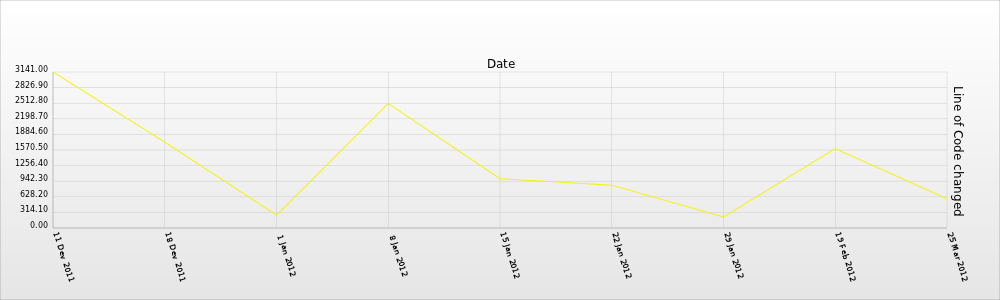
\includegraphics[width=\textwidth, keepaspectratio=true]{images/git_work_time.png}
  \caption{Work over time}
  \label{fig:git_work_time}
\end{figure}

Concurrent to this project, I assisted in the successful production of a wireless sensor network using
the ProSpeckz IIK (your ref) which contained a CC2420 IEEE 802.15.4 radio with a chip configuration
similar to that on the Respire (ref). Unlike the NRF24 radio, I had few difficulties programming the
CC2420 (at least in its configuration on the ProSpeckz IIK), even though it has a more complex
interface. Unfortunately the NRF24 radio is a fixed component of the Respire and could not be
replaced for testing of alternative radios. For TDMA to be applied successfully to a Respire network,
I am of the opinion that these problems with the NRF24 will have to be overcome. This has recently
become a greater priority for the Respire section of the Speckled Computing group at Edinburgh
University because they are reaching the limitations of the simpler type of wireless system currently
in use.


External to Edinburgh University, the NRF24 radio is currently used principally for use in wireless
keyboards and mice, with a maximum of 6 devices in each network. The recent family of Logitech
Unifying(r) devices, which allows these devices to to communicate with a single USB dongle, is one
of the NRF24’s largest known implementation. Within this type of configuration, devices do not need
to transition between transmit and receive states often and do not require synchronisation. I am
aware of two articles reporting successful implementation of a TDMA-based wireless sensor network
using the NRF24 family of radios (refs) in other devices, which suggest that it should be possible to
use it within the requirements of the Respire project. From the information included in these
publications, I could not identify any significant differences between their approach and mine to
programming the NRF24, although in both papers the NRF24L01 was used where as the Respire
contains the NRF24L01+. The stated difference between these two generations of NRF24 is that the
Respire version includes several hardware-accelerated networking features. I tested my system with
these features both enabled and disabled without any improvement.


(Analyzing Energy Consumption in a Gossiping MAC Protocol) and (Decentralized frame
synchronization of aTDMA-based wireless sensor network) REFS


\section{The Respire MCU}
The EFM32 appears to be an excellent choice for the Respire which, although not fully utilised in this
project, enables substantial power and lower energy improvements over the previous generations of
hardware. The consistency of the EMF32’s pin configurations throughout its family of chipsalso
allows the MCU in the Respire to be replaced without need for a redesigned circuit board. This was
an an active design choice, as it allows the future Respire to use the EFM32 Cortex-M4, soon-to-be-
released, again reducing energy needs whilst improving performance by use ofa hardware floating-
point unit. This design to enable future change of EFM32 has again been used to reduce the time to
market by both allowing the immediate use of the Cortex-M3 line, with knowledge of the later
compatibility, and by using a more powerful chip allowing over time with optimisations lower power
replacements. I would of wished this design desision had also extended towards the radio circuitry.

\section{Power Reductions}
By Utilising the low-powe 32Khz clock on the EFM32 my design tried aimed to provide minumin MCU
interation during the radio prosses. ...
About the code in the respire that reduces it power in general and aid development
Accuracy of the packet transmission time estimates

\section{Wireless Medical Devices and their Standardisation}

\subsection{Wireless Medical Device Standards}
At current there is no single standard for wireless medical equipment with many current viable
solutions. With each solution developed by competing organisations there is little sign that this
situation will change within the scope of the Respire project. It is however important when choosing
or developing a solution to review and analyse the competition.

\subsection{Bluetooth Lower Power}
The Bluetooth Special Interest Group and its Bluetooth standard is one of the most prevalent
Personal Area Networks (PAN) technologies. The next generation of the Bluetooth specification
includes a new Bluetooth Low Energy (BLE) sub-specification, specifically designed to address the
needs of sensor networks. BLE markedly reduces the power requirements for Frequency-hopping
spread spectrum that is prevalent in the full Bluetooth specification. BLE however has only just
become available with the recent finalisation of the standard, but it would be the most likely
alternative solution for the Respire.


\subsection{IEEE 802.15.4}
IEEE 802.15.4 provides a specification on many areas of a full wireless network, ranging from the
physical layer to the data to be sent over it. The broad approach of this specification has led to the
ZigBee standard, producing smaller more manageable standards to each application, including
health care. A second approach of managing the IEEE 802.15.5 specification has been to overlay the
IPv6 specification to produce 6LowPan.


\subsection{ANT}
ANT is a fully proprietary radio and network implementation designed to simplify the production of
wireless health care devices. As a recent and closed system, few devices have been produced
utilising its technology.


\subsection{\acf{ISM} Bands}
With the finite usable frequency ranges available to all wireless radio devices, and those devices that
emit radio interference, there are restrictive licensing systems in place. Licensing systems are
independently run by each country or region, but from 1980 a movement began to identify a set of
frequency bands that could be used worldwide without a licence \cite{ISMGen}.
With the introduction of the unlicensed (but still heavily restricted) \ac{IMS} bands,
communication via modern wireless equipment became a
widely-available possibility. A key 2.4 GHz band became the most popular for consumer electronics
communications due to its high bandwidth, long range and ability to pass through internal walls. This
convergence of signals into a single small band, , has created a crowded environment which,
compounded by the use of microwave ovens and other interference devices, needs powerful and
creative communication algorithms to penetrate and be reliable. The NRF24 uses Gaussian
frequency-shift keying to optimise throughput but does little to avoid interference. However it has
been shown that a frequency-hopping system to reduce the susceptibility to interference can be
implemented on the NRF24. (ref)


\section{Related Work}

\subsection{Edinburgh University}
Edinburgh University, under the leadership of J Mann, has also produced a separate implementation
of a radio interface for the Respire. This implementation was designed with power efficiency as the
only goal. To this end the system is designed such that the radio is only on, and only broadcasts
when data needs to be sent. This system therefore produces the most efficient power solution that
could be implemented on the device, ignoring optimisations of the design. The system also uses the
hardware accelerated ShockBurst\textregistered and MultiCeiver\textregistered system designed by Nordic Semiconductors.
With a brief of a fully managed network system suitable for hospital use, this design was decided not
to be suitable.Also by the extended use of the NRF24.the design has underused the features of the
EFM32. With the ability for asynchronously clocked serial transfer automated by and interrupts and
managed by the DMA not been utilised a similar chip could have been used.

\subsection{Alabama University}
To do

\section{Future Work}
I an attempt to improve the systems lower use it was found that the SPI connection to the radio is
under utilised by the use of a single buffer. I attempted To fix this issue with the use of the double
buffer but was unsuccessful due to a hardware flaw in the EFM32 (ref needed), where if the double
buffer and single buffer are used in the same application it is not reflected in the status of the buffer
free register. The issue was not overcome by the prescribed fix as the initial issue absorbed the time
allocated for the feature and therefore would be a good candidate for improving the system’s
energy use. A secondary, and preferred, final solution for longer transfers would be to enable the
DMA and fully enable the EFM32 to power down the entire length of the transfer. I decided that the
DMA solution was out with the time constraints afforded to this section of the project and therefore
would also be a key step in improving the system’s energy usage.
As many people believe strongly in their privacy, especially when concerning their medical records, it
should be considered if cryptography should be implemented on the system. This feature should not
impose as big an effect on the energy efficiency as most devices as the EFM32 has hardware
accelerated encryption, however it does not include any acceleration for hashes.


